\chapter{الميكروبات والعدوى}\label{ch:g9:microbes-and-infection}

ما زالت تظلل هذا الكتاب منذ \omterm{def:g1:healthy-habits:germs}{جراثيم} السنة الأولى غير
المرئية (\cref{def:g1:healthy-habits:germs}): فارتقت إلى
يد عاملة في المخبزة (\cref{ch:g6:producing-our-food})،
وإلى أطقم محللة في \omterm{def:g6:decomposers-and-soil:soil}{التربة}، وإلى خصم يتطور في جناح
المستشفى (\cref{ex:g9:how-species-change:resistance}).
وهذا الفصل يوفي \omterm{def:g6:producing-our-food:fermentation}{الميكروبات} حسابها كاملًا أخيرًا: ما هي،
وكيف تهاجم الأقلية الضارة، وكيف تمسك دفاعات الجسم
الخارجية --- ودفاعاتنا نحن --- الأبواب.

\section{عالم الميكروبات}

\begin{definition}[الميكروبات، مفروزة]\label{def:g9:microbes-and-infection:sorted}
\emph{الكائنات المجهرية}\index{كائن مجهري} ---
\omterm{def:g6:producing-our-food:fermentation}{الميكروبات} --- كائنات حية أصغر من أن ترى \omterm{def:g1:the-five-senses:sense}{بالعين} المجردة.
وأهم أنواعها:
\begin{itemize}
  \item \emph{البكتيريا}\index{بكتيريا}: \omterm{def:g5:first-look-at-cells:cell}{خلايا} مفردة بلا
        \omterm{def:g6:cell-unit-of-life:parts}{نواة} حقيقية، أصغر بكثير من خلاياك، وتنقسم سريعًا
        (عالم
        \cref{def:g6:cell-unit-of-life:unicellular}) ---
        في كل مكان، وبأعداد تفوق العد؛
  \item \emph{\omterm{def:g6:decomposers-and-soil:decomposers}{الفطريات} وحيدة \omterm{def:g5:first-look-at-cells:cell}{الخلية} وغيرها}: الخمائر
        (\cref{ex:g6:producing-our-food:bread})، \omterm{def:g4:plants-without-seeds:spore}{وأبواغ}
        العفن، وسابحات قطرة البركة؛
  \item \emph{الفيروسات}\index{فيروس}: أصغر بعد، ومختلفة
        في \omterm{def:g5:biodiversity:species}{النوع} --- قصاصة معبأة من نص وراثي (أحرف
        \cref{def:g9:genes-and-dna:dna}) في معطف، \emph{لا
        \omterm{def:g5:first-look-at-cells:cell}{خلية} لها ولا حياة خاصة بها}: فالفيروس لا يفعل
        شيئًا حتى يدخل \omterm{def:g5:first-look-at-cells:cell}{خلية} حية فيحول آلة قراءتها إلى نسخ
        نص الدخيل. وعلى علامات
        \cref{prop:g1:living-or-not:signs}، تقف الفيروسات
        على حافة الحياة تمامًا.
\end{itemize}
\end{definition}

\begin{proposition}[غير ضارة في أكثرها، وضرورية في كثير منها]\label{prop:g9:microbes-and-infection:mostly}
السمعة الضارة تقرير أقلية. فأكثر \omterm{def:g6:producing-our-food:fermentation}{الميكروبات} تتجاهلنا؛
وكثير منها يخدمنا: أطقم \omterm{prop:g6:decomposers-and-soil:decomposition}{التحلل}
(\cref{def:g6:decomposers-and-soil:decomposers})،
والأيدي العاملة في الغذاء، وكيميائيو \omterm{def:g6:decomposers-and-soil:soil}{التربة} ---
و\emph{نبيتك المقيم}\index{نبيت مقيم} أنت: تريليونات
\omterm{def:g9:microbes-and-infection:sorted}{البكتيريا} غير الضارة تفرش \omterm{def:g1:the-five-senses:sense}{الجلد} والمعي، تعين على \omterm{def:g4:journey-of-food:digestion}{الهضم}،
وتزاحم الدخلاء عن الأرض بمجرد احتلالها. ولا يسبب المرض
إلا أقلية صغيرة --- هي \emph{الممرضات}\index{ممرض}.
\end{proposition}
\admitted

\begin{example}[جسم واحد، وثلاث علاقات]\label{ex:g9:microbes-and-infection:relations}
على جلدك في هذه الدقيقة: مقيمون بالمليارات، يمسكون
السطح (العلاقة الأولى: تحالف). وفي لبنك على الفطور:
عمال، يحمّضون بأمر (العلاقة الثانية: توظيف،
\cref{ex:g6:producing-our-food:yogurt}). وعلى المسمار
الصدئ في الحظيرة: \omterm{def:g4:plants-without-seeds:spore}{أبواغ} \omterm{def:g9:microbes-and-infection:sorted}{بكتيريا} الكزاز، تنتظر جرحًا
عميقًا (العلاقة الثالثة: أقلية \omterm{prop:g9:microbes-and-infection:mostly}{الممرضات}، وسبب
\cref{ch:g9:immune-defenses} وجرعة الكزاز المعزّزة).
\end{example}

\section{العدوى: الهجوم، مرحلة مرحلة}

\begin{definition}[مراحل العدوى]\label{def:g9:microbes-and-infection:stages}
\emph{العدوى}\index{عدوى} تجري في مراحل، لكل واحدة
اسمها:
\begin{enumerate}
  \item \emph{الانتقال}: يسافر الممرض --- بالأسطح
        الملموسة والأيدي، وبرذاذ السعال، وبالطعام والماء
        الملوثين، وبالدم، وبالطريق الجنسي الذي أشار إليه
        \cref{def:g8:contraception:condom}؛
  \item \emph{الدخول}: عبر ثغرة --- \omterm{def:g1:the-five-senses:sense}{جلد} مقطوع، أو أبواب
        الجسم المفتوحة: المسالك الهوائية، والمعي، والطرق
        السابقة؛
  \item \emph{التضاعف}: في الدفء \omterm{def:g6:exploring-our-environment:conditions}{والرطوبة} والغذاء، ينقسم
        الواصلون --- \omterm{def:g9:microbes-and-infection:sorted}{البكتيريا} وفق قاعدة \omterm{def:g6:exploring-our-environment:conditions}{الشروط} في
        \cref{prop:g6:decomposers-and-soil:speed}، تضاعف
        أعدادها في ساعات؛ \omterm{def:g9:microbes-and-infection:sorted}{والفيروسات} بتحويل \omterm{def:g5:first-look-at-cells:cell}{الخلايا} إلى
        مطابع نسخ؛
  \item \emph{المرض}: الأعراض --- من الضرر نفسه، ومن
        سموم \omterm{def:g9:microbes-and-infection:sorted}{البكتيريا}، وجزئيًا (في الفصل التالي) من
        معركة الدفاع ذاته.
\end{enumerate}
\end{definition}

\begin{example}[غازيان، متقابلان]\label{ex:g9:microbes-and-infection:contrast}
\omterm{def:g9:microbes-and-infection:sorted}{بكتيريا} الجرح في مقابل \omterm{def:g9:microbes-and-infection:sorted}{فيروس} زكام الشتاء. \omterm{def:g9:microbes-and-infection:sorted}{البكتيريا}:
تدخل من الثغرة، وتتضاعف \emph{بين} \omterm{def:g5:first-look-at-cells:cell}{الخلايا} في النسيج
الدافئ الرطب، وفضلاتها تسمم الجوار --- وهو خفقان الإصبع
المتقيح وقيحه. \omterm{def:g9:microbes-and-infection:sorted}{والفيروس}: يركب رذاذة إلى بطانة المسالك
الهوائية، ويدخل \omterm{def:g5:first-look-at-cells:cell}{خلايا} البطانة نفسها، فتطلق كل \omterm{def:g5:first-look-at-cells:cell}{خلية}
مخطوفة حشدًا من النسخ قبل أن تخفق --- وهو خشونة الحلق
وسيلان الأنف في أثره. آليتان مختلفتان؛ فالمضاد الحيوي
الذي يجوّع الأول لا يمس الثاني، لأن الثاني يستعير آلتك
\emph{أنت}، والأدوية ضده صعبة التصويب.
\end{example}

\section{إمساك الأبواب}

\begin{proposition}[الدفاعات الأولى]\label{prop:g9:microbes-and-infection:doors}
قبل أي معركة، يمسك الجسم حدوده:
\begin{itemize}
  \item \emph{\omterm{def:g1:the-five-senses:sense}{الجلد}}: جاف، متطبق، يجدد نفسه --- وهو
        السور (عضو \cref{def:g1:the-five-senses:sense}،
        في مهمة حراسة)؛
  \item \emph{البطانات ومكانسها}: أسطح تنظيف المسالك
        الهوائية
        (\cref{prop:g7:lungs-and-gas-exchange:smoke}
        بيّنها محمّلة فوق طاقتها)، وكيمياء الشطف في الدمع
        \omterm{def:g4:journey-of-food:tract}{واللعاب}، وحمّام \omterm{def:g4:journey-of-food:tract}{المعدة} الحمضي
        (\cref{pb:g7:digestion-and-nutrients:1} يعقّم وهو
        يهضم)؛
  \item \emph{المقيمون}: أرض النبيت المحتلة، ولا مكان
        كبيرًا للهبوط؛
\end{itemize}
\omterm{def:g1:healthy-habits:hygiene}{والنظافة} تمدّها: صابون
\cref{met:g1:healthy-habits:hands} (ومعه الآن آليته
الكاملة --- الانتقال مقطوعًا)، والماء المأمون، والطعام
المطهو والمحفوظ باردًا (رفض \omterm{def:g6:exploring-our-environment:conditions}{الشروط} في
\cref{rem:g6:producing-our-food:goodbad})، والإبرة
المعقّمة، وحاجز \omterm{def:g8:contraception:condom}{الواقي}. وكل قاعدة \omterm{def:g1:healthy-habits:hygiene}{نظافة} في هذا الكتاب هي
مرحلة انتقال أو دخول، مسدودة.
\end{proposition}
\admitted

\begin{omfigure}
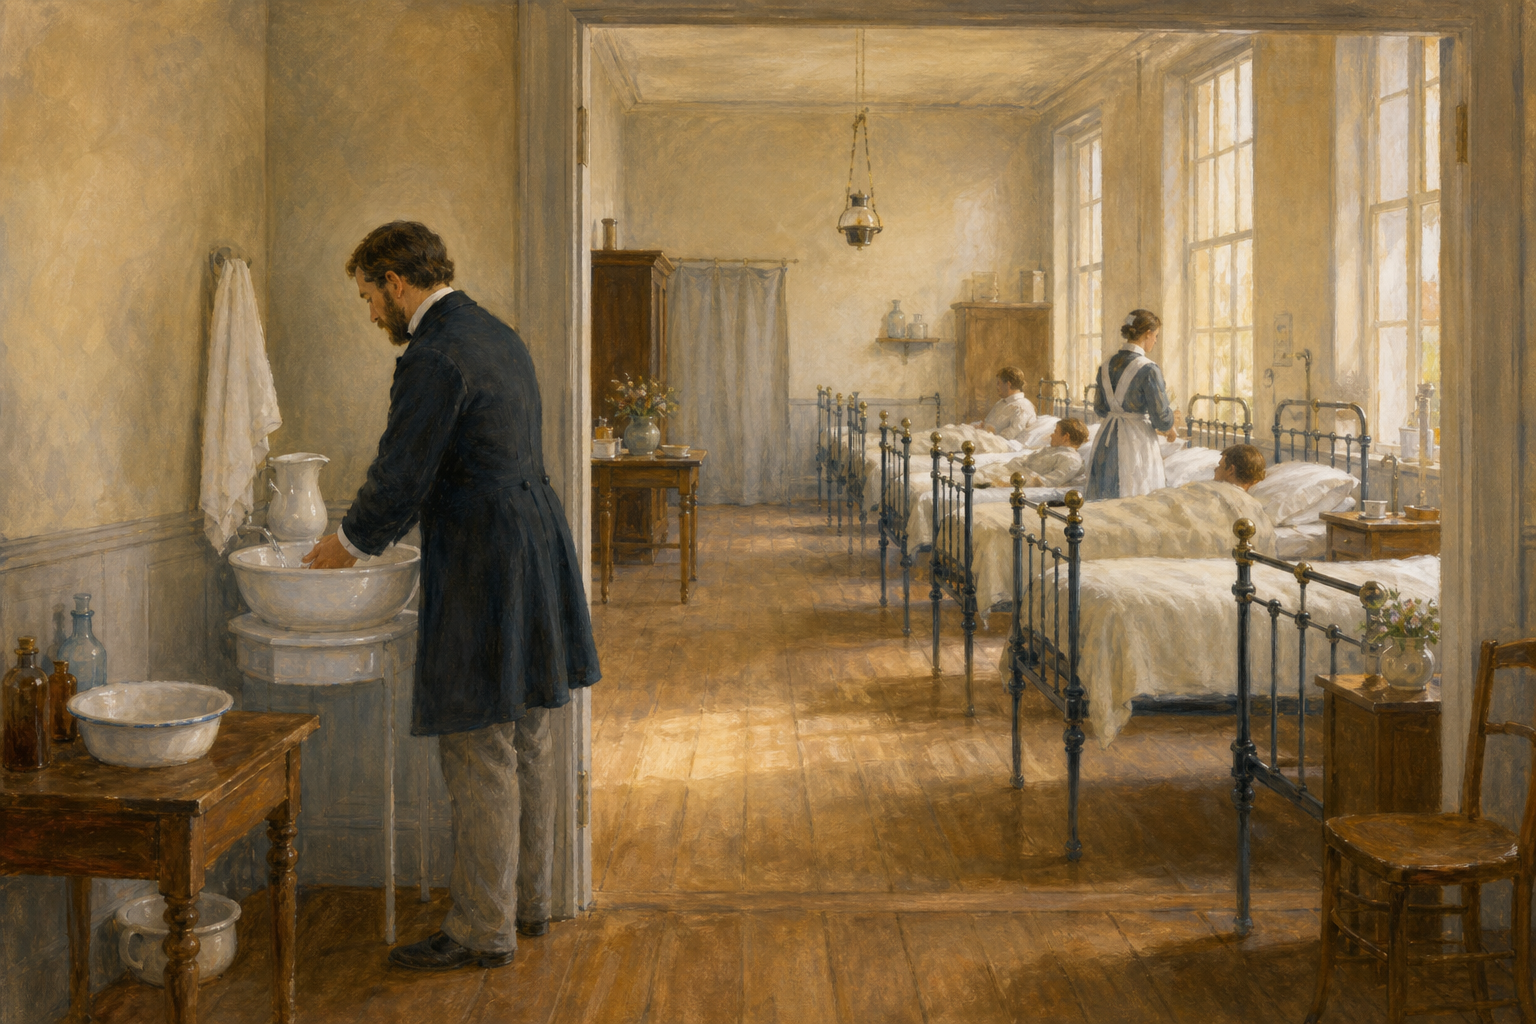
\includegraphics[width=0.6\linewidth]{images/book1/ai/g9-microbe-washing.png}

{\small أرخص دواء في التاريخ: مغسلة عند باب الجناح، تقطع
على سعاة لا تراهم \omterm{def:g1:the-five-senses:sense}{عين}.}
\end{omfigure}

\begin{example}[الطبيبان اللذان حركا الأرقام]\label{ex:g9:microbes-and-infection:history}
اسمان يثبّتان الحكاية. سيميلفايس، في فيينا أربعينيات
القرن التاسع عشر: انهارت وفيات حمى النفاس في جناح
\omterm{def:g2:born-grow-die:cycle}{الولادة} عنده حين غسل الأطباء أيديهم بين غرفة التشريح
وقاعة الوضع --- فقطع الانتقال قبل أن يكون أحد قد رأى
المسافر. ثم بيّن باستور بعد جيل المسافرين أنفسهم:
\omterm{def:g6:producing-our-food:fermentation}{ميكروبات}، لا ``هواء فاسد''، تحمّض النبيذ، وتقتل دود
الحرير، وتصيب الجروح --- والحرارة (\emph{بسترته}) أو
التعقيم توقفها. وقد حوّلت نظرية \omterm{def:g1:healthy-habits:germs}{الجراثيم} المستشفيات من
أخطار إلى دفاعات في مدى عمر واحد.
\end{example}

\begin{omfigure}
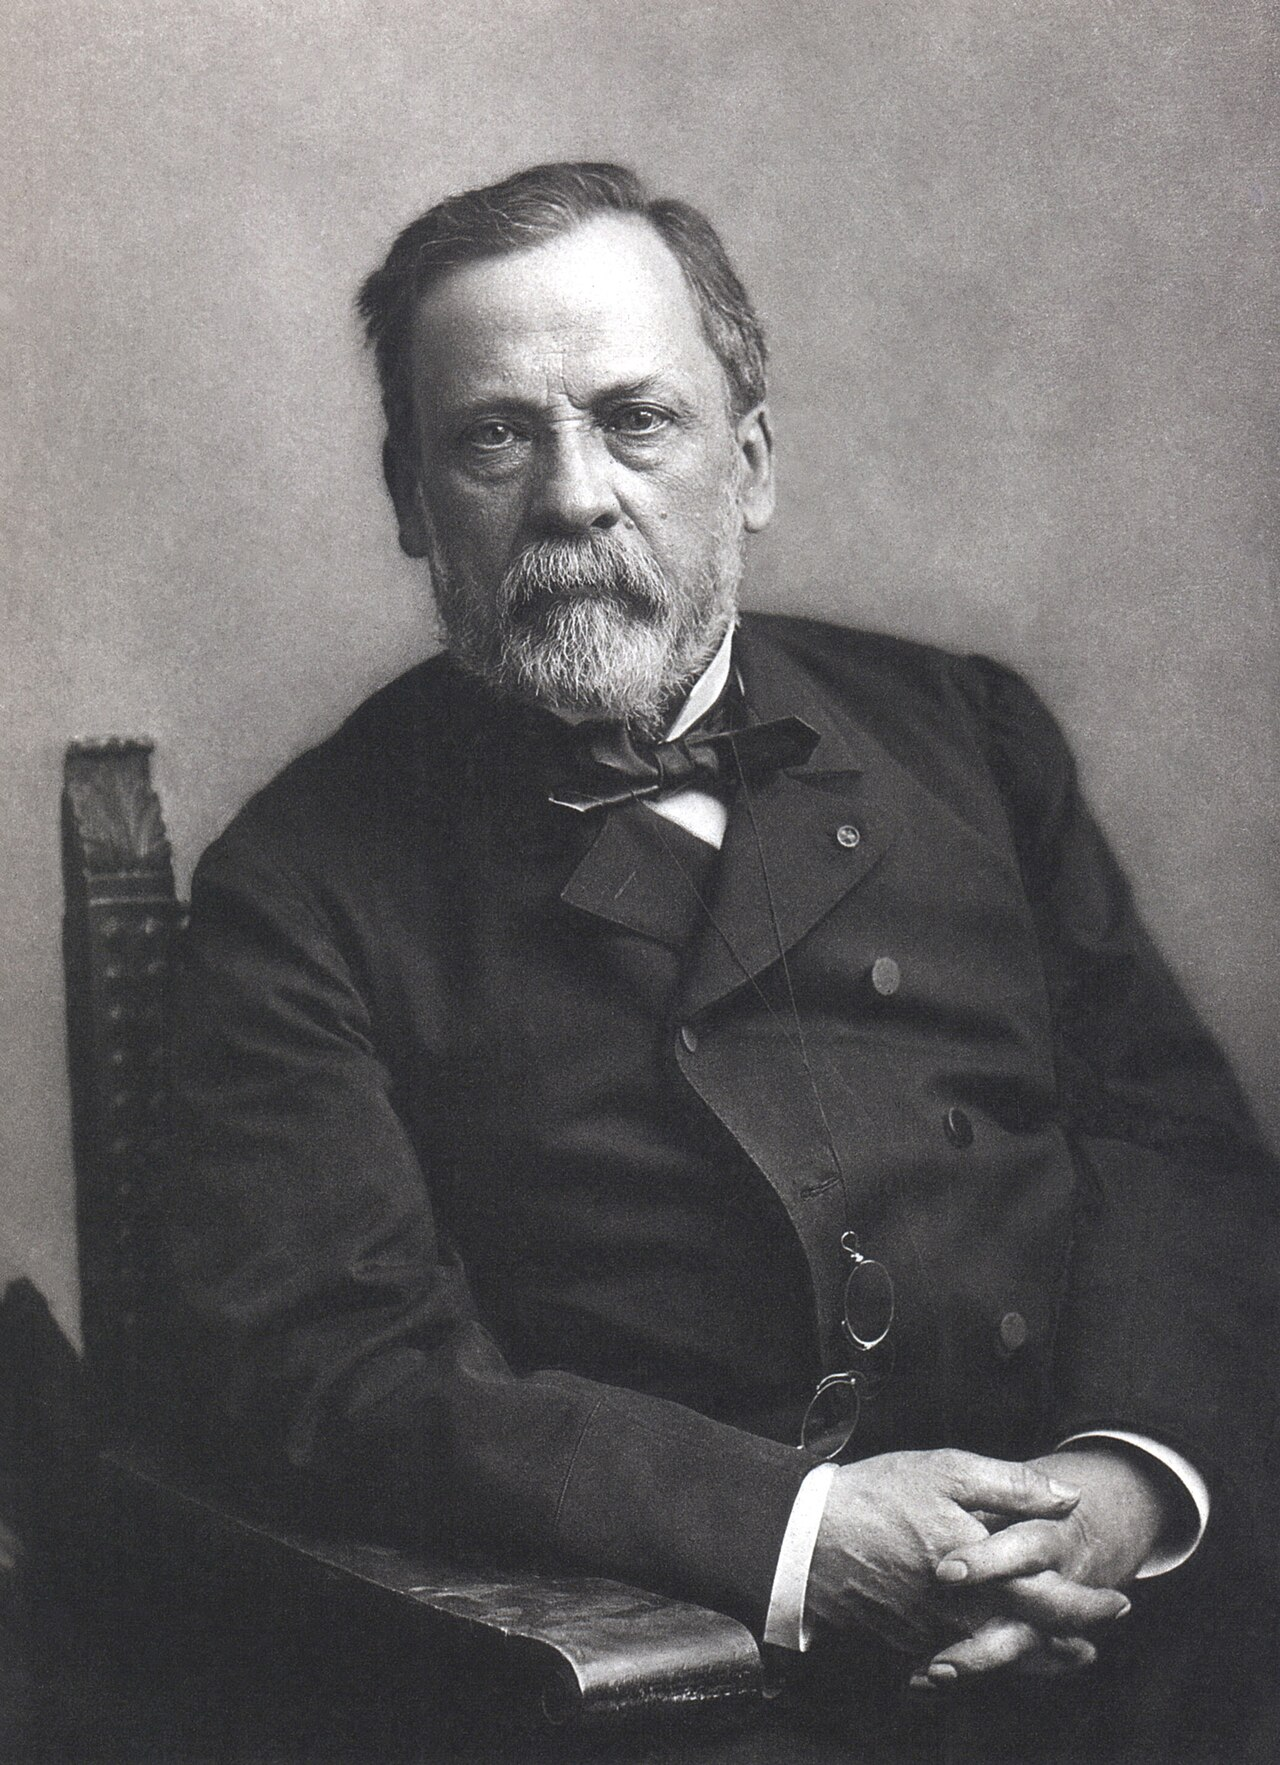
\includegraphics[width=0.42\linewidth]{images/book1/pasteur.jpg}

{\small لويس باستور، مصورًا بعدسة بول نادار: العالم الذي
بيّن المسافرين غير المرئيين أنفسهم.}
\end{omfigure}

\begin{method}[تدقيق خطر عدوى]\label{met:g9:microbes-and-infection:audit}
في أي موقف --- مطبخ، أو جرح، أو جناح، أو حشد:
\begin{enumerate}
  \item سمّ الممرض المحتمل ونوعه (\omterm{def:g9:microbes-and-infection:sorted}{بكتيريا}، أو \omterm{def:g9:microbes-and-infection:sorted}{فيروس}، أو
        \omterm{def:g6:decomposers-and-soil:decomposers}{فطر})؛
  \item وتتبع طريق انتقاله إليك؛
  \item وجد باب دخوله؛
  \item واسأل ما الذي يضاعفه --- الدفء، \omterm{def:g6:exploring-our-environment:conditions}{والرطوبة}،
        والغذاء، والوقت؛
  \item واسدد أرخص مرحلة: اغسل، واطه، وغطِّ، وبرّد،
        وعقّم، ولقّح
        (\cref{ch:g9:immune-defenses} يشرح الأخيرة).
\end{enumerate}
\end{method}

\section{تمارين}

\begin{exercise}[$\star$]\label{exo:g9:microbes-and-infection:1}
سمّ \omterm{def:g5:biodiversity:species}{أنواع} \omterm{def:g6:producing-our-food:fermentation}{الميكروبات} الرئيسة، وما الذي يميز \omterm{def:g9:microbes-and-infection:sorted}{الفيروسات}.
\end{exercise}

\begin{exercise}[$\star$]\label{exo:g9:microbes-and-infection:2}
ما \omterm{prop:g9:microbes-and-infection:mostly}{النبيت المقيم}، وأي خدمتين يقدمهما؟
\end{exercise}

\begin{exercise}[$\star$]\label{exo:g9:microbes-and-infection:3}
اذكر مراحل \omterm{def:g9:microbes-and-infection:stages}{العدوى} الأربع بمثال لكل واحدة.
\end{exercise}

\begin{exercise}[$\star$]\label{exo:g9:microbes-and-infection:4}
قابل بين الجرح المتقيح والزكام: أين يتضاعف كل غاز؟
\end{exercise}

\begin{exercise}[$\star$]\label{exo:g9:microbes-and-infection:5}
سمّ أربعًا من الدفاعات الأولى والمرحلة التي تمسكها كل واحدة.
\end{exercise}

\begin{exercise}[$\star$]\label{exo:g9:microbes-and-infection:6}
ما الذي قطعه غسل أيدي سيميلفايس، وما الذي أضافه باستور؟
\end{exercise}

\begin{exercise}[$\star\star$]\label{exo:g9:microbes-and-infection:7}
لماذا تترك المضادات الحيوية الزكام من غير مساس؟ أجب
بآليتي الغازيين.
\end{exercise}

\begin{exercise}[$\star\star$]\label{exo:g9:microbes-and-infection:8}
أعد استنباط ثلاث قواعد \omterm{def:g1:healthy-habits:hygiene}{نظافة} من \omterm{def:g3:stages-of-life:stages}{الطفولة}
(\cref{ch:g1:healthy-habits}) بوصفها سدودًا لمراحل، مع
تسمية الآلية.
\end{exercise}

\begin{exercise}[$\star\star$]\label{exo:g9:microbes-and-infection:9}
طبّق \cref{met:g9:microbes-and-infection:audit} على سلطة
دجاج في نزهة صيفية، دفئت في سيارة ثلاث ساعات.
\end{exercise}

\begin{exercise}[$\star\star$]\label{exo:g9:microbes-and-infection:10}
لماذا يهم غسل اليدين \emph{بين} المهام أكثر من غسلهما
كثيرًا؟ (جناح سيميلفايس يملك الجواب.)
\end{exercise}

\begin{exercise}[$\star\star$]\label{exo:g9:microbes-and-infection:11}
ضع جناح \cref{ex:g9:how-species-change:resistance} في
هذا الفصل: أي مرحلة يهاجم المضاد الحيوي، وماذا يربّي
استعماله المهلهل؟
\end{exercise}

\begin{exercise}[$\star\star\star$]\label{exo:g9:microbes-and-infection:12}
``\omterm{def:g9:microbes-and-infection:sorted}{الفيروس} نص يستعير مطبعة.'' افتح الصورة بمساعدة
\cref{def:g9:genes-and-dna:dna}
و\cref{def:g9:microbes-and-infection:sorted} ---
واستعملها لتقول لماذا تقف \omterm{def:g9:microbes-and-infection:sorted}{الفيروسات} على حافة الحياة،
ولماذا يصعب تدويتها.
\end{exercise}

\section{مسألة: دفتر الفاشية}

\begin{problem}[{مسألة نهاية الأسبوع --- فاشية مدرسية،
متتبعة مرحلة مرحلة}]\label{pb:g9:microbes-and-infection:1}
فاشية مدرسية (متخيَّلة): في أسبوع واحد يبلّغ نصف الصف
التاسع ب عن حمى وسعال؛ ثم تتناثر الحالات في الصفوف
الأخرى. وتمسك ممرضة المدرسة دفتر فاشية وتطلب من صف
البيولوجيا أن يعينها على قراءته.

\medskip\noindent\textbf{الجزء الأول --- قراءة الانتشار.}
\begin{enumerate}
  \item الحالة الأولى --- حالة الدليل --- كانت في التاسع
        ب؛ والثماني التالية يشاركنها صفها ورفيقاتها في
        كرة الطاولة. سمّ طريق الانتقال المرجح، وباب
        الدخول.
  \item تتضاعف الحالات كل يومين في البداية. حساب أي
        مرحلة يظهر، وآلة من تقوم بالنسخ إن كان العامل
        فيروسًا؟
  \item قائمة الممرضة: بداية الحمى، والسعال، وخشونة
        الحلق. أي مرحلة تعلّمها الأعراض، ومن أي مصدرين
        تنشأ؟
  \item ولماذا قفزت الفاشية بين الصفوف عند اجتماعي
        المدرسة العامّين في ذلك الأسبوع بالضبط؟
\end{enumerate}

\medskip\noindent\textbf{الجزء الثاني --- الهجوم المضاد.}
\begin{enumerate}[resume]
  \item إجراءات المدرسة: التلاميذ المرضى إلى بيوتهم؛
        والنوافذ تفتح (\cref{exo:g4:breathing:10})؛ وغسل
        الأيدي يدرَّب؛ والمعدات المشتركة تمسح. أسند لكل
        إجراء المرحلة التي يسدها.
  \item يطالب ولي أمر بمضادات حيوية للجميع. اكتب مسودة
        جواب الطبيب في فاشية فيروسية --- وتحذير الانتقاء
        (\cref{exo:g9:how-species-change:10}) لو نثرت
        المضادات مع ذلك.
  \item ويبلّغ المقصف في الوقت نفسه عن حالتي \omterm{def:g4:journey-of-food:tract}{معدة} تتبعان
        إلى حلوى لم تبرَّد. دقّق تلك الفاشية الجانبية وفق
        \cref{met:g9:microbes-and-infection:audit} ---
        \omterm{def:g5:biodiversity:species}{نوع} عامل مختلف، ومراحل مختلفة.
  \item ولماذا ترسم الممرضة \emph{من جلس أين} بدل أن
        تعامل الحالات على أنها عشوائية؟ وما خريطة
        الفاشية، بلغة الانتقال؟
\end{enumerate}

\medskip\noindent\textbf{الجزء الثالث --- المراجعة.}
\begin{enumerate}[resume]
  \item اكتب سيرة الفاشية في المراحل الأربع، من حالة
        الدليل إلى الخمود.
  \item خمدت الفاشية قبل أن تبلغ كل تلميذ. اعرض آليتين
        --- سدود الإجراءات، وإشارة الفصل التالي: من
        كانوا منيعين سلفًا من سلالة العام الماضي
        القريبة.
  \item وأضف فقرة التاريخ: أي درسين من القرن التاسع عشر
        (\cref{ex:g9:microbes-and-infection:history})
        انحدرت منهما استجابة المدرسة كلها؟
  \item واختم الدفتر بمنهج التدقيق شعارًا: جملة واحدة عن
        أين يكون إيقاف الفاشيات أرخص ما يكون.
\end{enumerate}
\end{problem}
